\clearpage
\section{Close proximity detection and navigation}
The close proximity system consists of two main components, one part that is reading from the ultrasonic sensors and another one for controlling the rover using the motor controller.

The ultrasonic sensors return distance measurements to the algorithm that then determines the optimal direction according to some threshold distances and different parameters.

\begin{figure}[H]
	\centering
	\begin{subfigure}[H]{0.4\textwidth}
		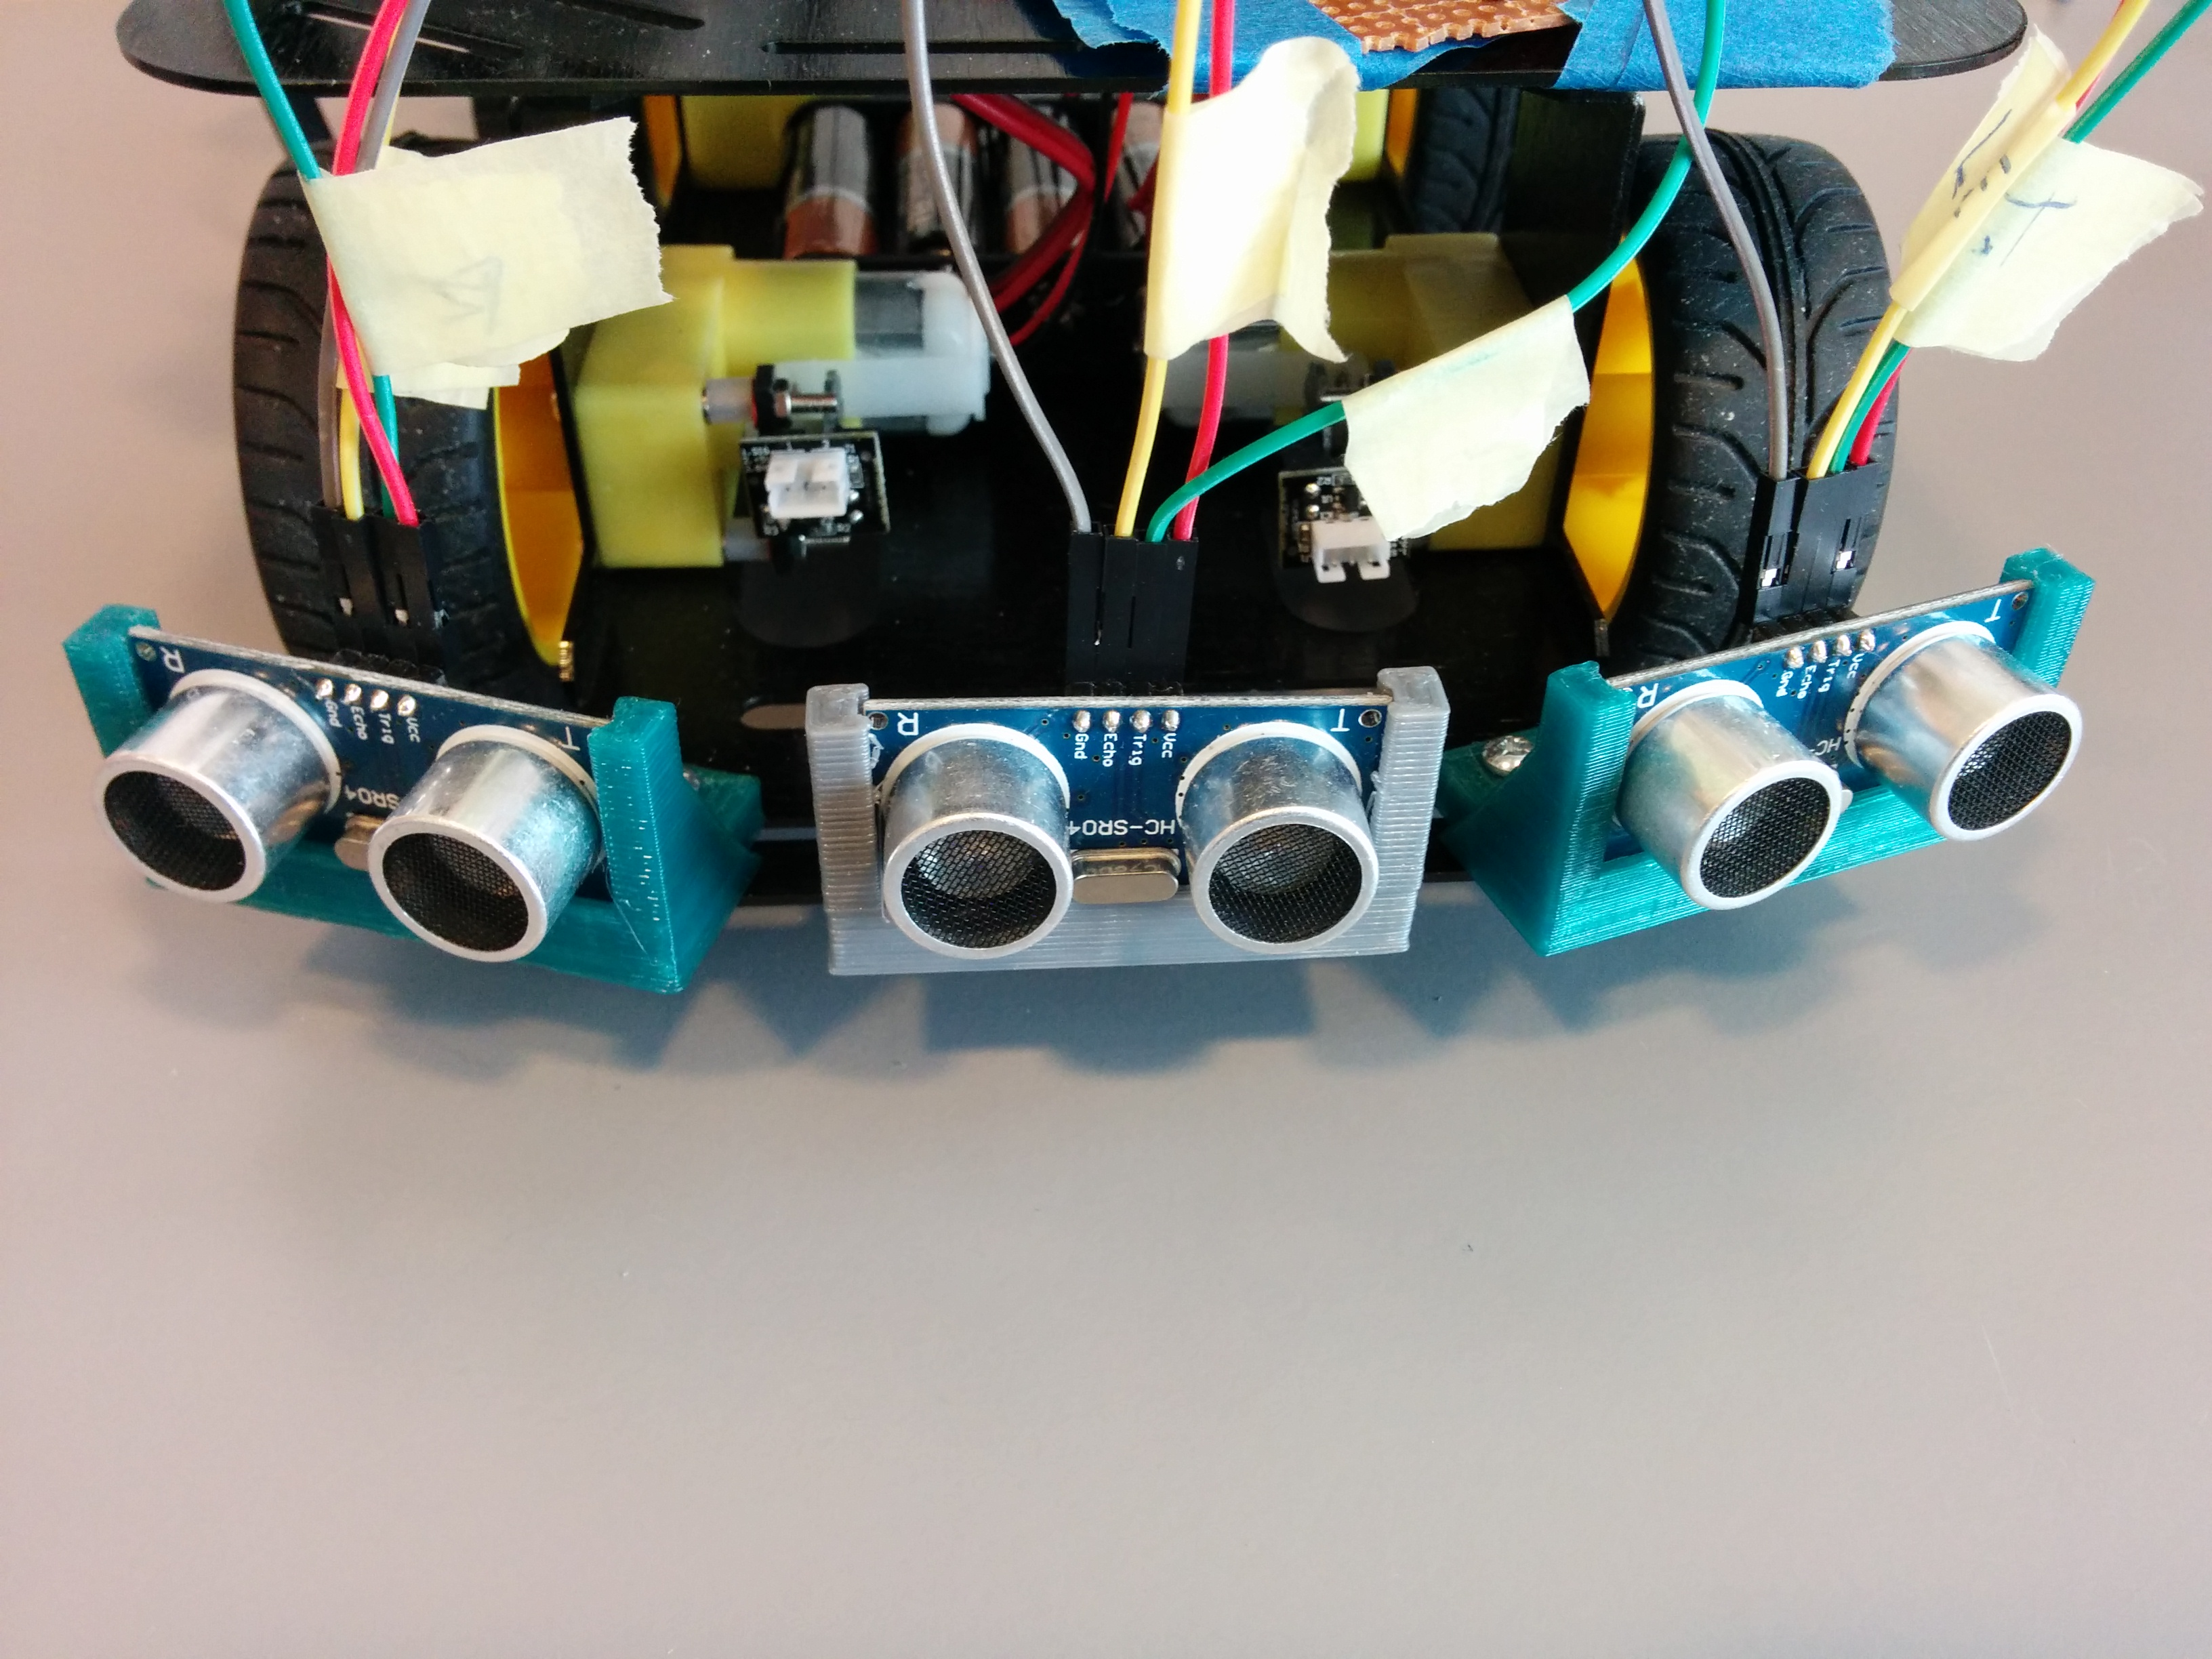
\includegraphics[width=\textwidth]{images/mounted_ultrasonic_sensors.jpg}
		\subcaption{The mounted sensors}
		\label{mounted_ultrasonicsensors}
	\end{subfigure}%
	\quad
	\begin{subfigure}[H]{0.4\textwidth}
		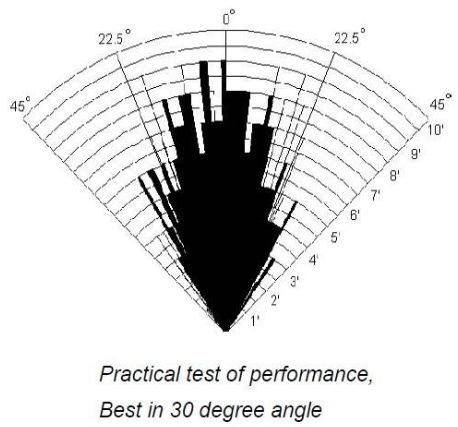
\includegraphics[width=\textwidth]{images/hcsr04angle.png}
		\subcaption{The measuring angle}
		\label{measuringangle}
	\end{subfigure}
\end{figure}

The current vision of the rover, which relies on the distance measurements from the sensors above, is limited to three different measurements. This unfortunately results in some blind spots between the ultrasonic sensors.
The ultrasonic sensor performs best at a $30\degree$ reading angle. This angle helps determine the area of which the ultrasonic sensor can read upon. The larger the angle, the less of a blind spot there will be between two ultrasonic sensors, depending on how they are mounted on the rover\cite{hcsr40datesheet}. Besides the $30\degree$ models there also exists the same ultrasonic sensors with a measuring angle of $15\degree$.

\clearpage
\begin{figure}[H]
	\centering
	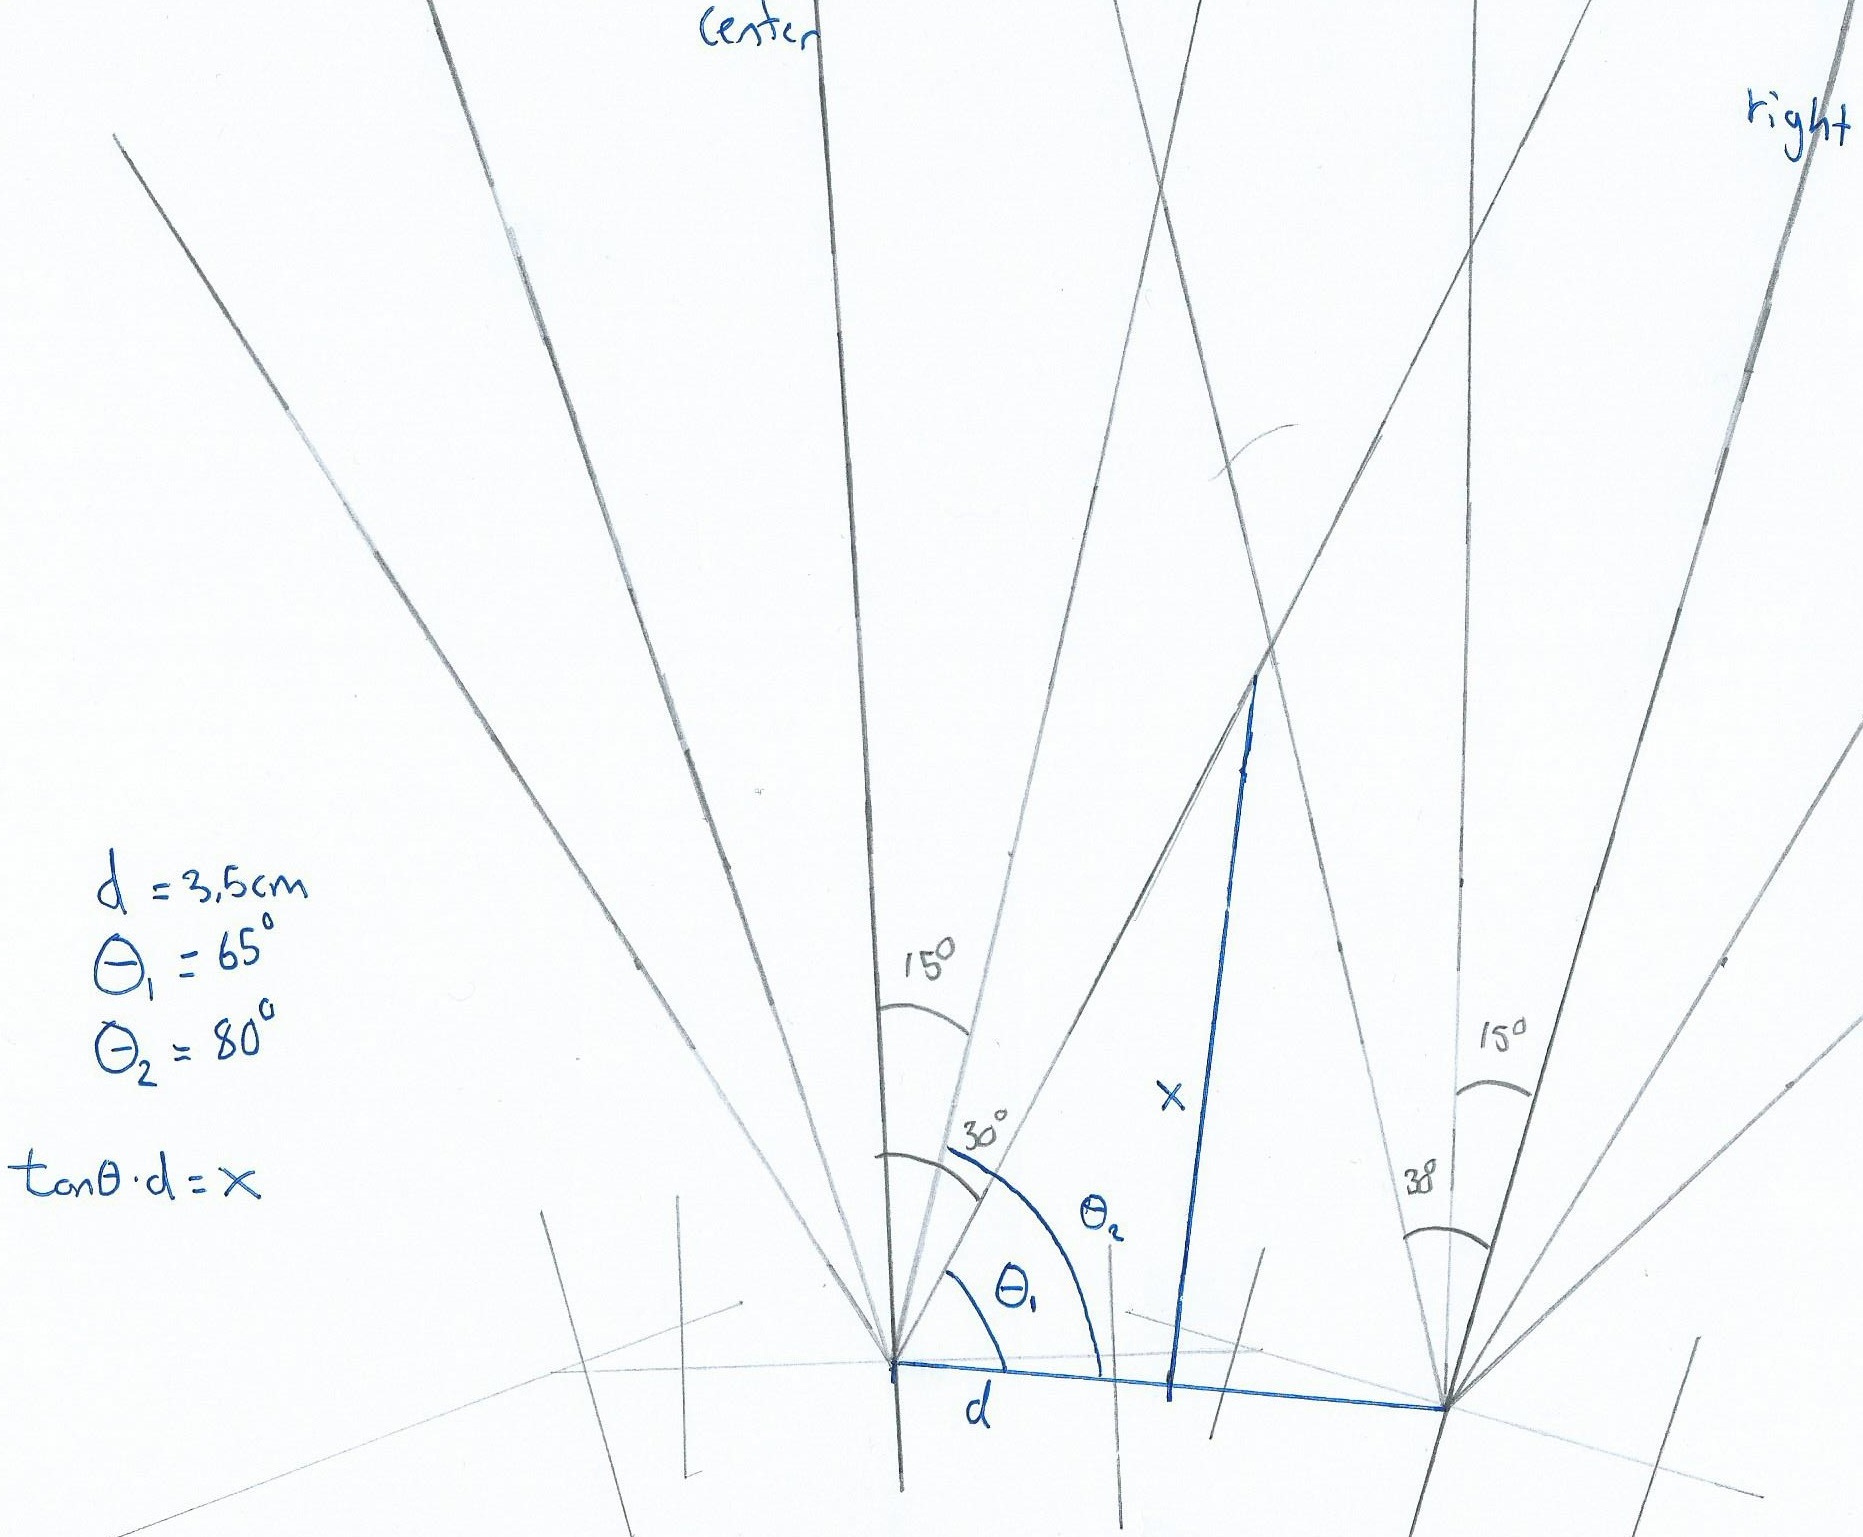
\includegraphics[width=0.8\linewidth]{images/blindspot_calc.jpg}
	\caption{The diagram used for the calculations}
	\label{calculationdiagram}
\end{figure}

The blind spot can be determined by finding the length $x$ on the figure above. The triangles with d as their bottom line indicate the area of which the ultrasonic sensors covers, for both the $15\degree$ and $30\degree$ measuring angles. Since some versions of the ultrasonic sensor perform best at an $15\degree$ angle, two different calculations have been made to help determine where the blind spots for this particular setup are located.
The length $x$ marked on the sketch above indicates where the blind spot starts. To find the length $x$, the equation $tan(\Theta)d = x$ can be used to solve the problem. The length d is found by taking half of the length between the center of each ultrasonic sensor and it this length stays constant for both measuring angle cases. $\Theta$ is found my measuring the angle between the length d and the measuring angle of the ultrasonic sensors. Since the ultrasonic sensors measuring angle is different for the two cases, the value of $\Theta$ changes depending on the ultrasonic sensors operates at $30\degree (\Theta_1)$ or $15\degree (\Theta_2)$.

$\Theta_1 = 65\degree$\quad\quad$d = 3.5cm$\quad\quad$tan(65\degree)3.5cm =  7.506cm$\\
$\Theta_2 = 80\degree$\quad\quad$d = 3.5cm$\quad\quad$tan(80\degree)3.5cm =  19.849cm$

The rover has two theoretical blind spots on either side of the center mounted ultrasonic sensors at a measuring angle of $15\degree$ the blind spot is $34.7cm^2$ and at $30\degree$ the blind is $13.1cm^2$. 

During testing these measurements will be used to figure out what the specific measuring angle is of the ultrasonic sensors the rover is equipped with, to help identify possible issues that might occur with how it operates.

\clearpage
\lstinputlisting[firstline=143, lastline=172, title=main, language=Python]{../code/autonomous-rover/obstacle-avoidance-args.py}

The core idea behind the current algorithm, is that every loop of the code, the three ultrasonic sensors mounted on the front of the vehicle all gather three separate measurements. Then afterwards the measurements are compared in three different statements that will determine the next direction the rover will be heading in. If the distance recorded by the left most facing ultrasonic sensor is less than the threshold distance set as the variable \textit{avoid\_at}, the rover will then turn towards the right for the amount of seconds that the \textit{turn\_time} variable is set to. The same thing applies to the ultrasonic sensor facing to the right, but instead the rover turns to the left when the threshold is exceeded.
If the threshold distance is exceeded at the center ultrasonic sensor, it determines whether the optimal path is to turn left or right depending on which direction has the largest distance measurement. This means that if an object is detected by the center ultrasonic sensor, the rover will then determine whether the distance measured to the left is greater than the distance measured to the right. The rover will then turn in the direction in which the distance measurement is greatest, since this in theory means that the rover will have the capability of travelling for a longer distance until meeting a new object that needs to be avoided or maneuvered around.\\


\lstinputlisting[firstline=31, lastline=49, title=getdist(), language=Python]{../code/autonomous-rover/triple-ultrasonic-test.py}

At the start of the navigation loop seen in the \textit{main} code, the \textit{getdist()} function is run three separate times with different arguments for each of the ultrasonic sensors. Measurements are gathered every 200ms, to allow the rover to move a short distance before re-calculating its direction. The datasheet for the ultrasonic sensors recommend a measurements cycle of at least 60ms, to ensure that the ultrasonic bursts do not overlap. In the appendix the full code can be found, where the arguments are clearly labelled to help determine what measurement is coming from what ultrasonic sensor (Appendix \ref{code:proximity-full}).